\icmltitle{Supplementary Material: \papertitle}

\icmlsetsymbol{equal}{*}

\begin{icmlauthorlist}
\icmlauthor{Alvaro Sanchez-Gonzalez}{dm}
\icmlauthor{Nicolas Heess}{dm}
\icmlauthor{Jost Tobias Springenberg}{dm}
\icmlauthor{Josh Merel}{dm}
\icmlauthor{Martin Riedmiller}{dm}
\icmlauthor{Raia Hadsell}{dm}
\icmlauthor{Peter Battaglia}{dm}
\end{icmlauthorlist}

\icmlaffiliation{dm}{DeepMind, London, United Kingdom}


\vskip 0.3in


\section{Summary of prediction and control videos}
\begin{table}[hb]
\caption{Representative trajectory prediction videos. Each shows several rollouts from different initial states for a single model trained on random control inputs. The labels encode the videos' contents: [\textbf{P}rediction/\textbf{C}ontrol].[\textbf{F}ixed/\textbf{P}arameterized/System~\textbf{I}D].[(System abbreviation)]}
\label{sm:table:rollouts}
\begin{center}
\begin{small}
\begin{tabular}{p{27mm}lll}
\toprule
 & Fixed & Parametrized & System ID \\
\midrule
Pendulum  & 
\href{\rolloutspendulum}{\rolloutspendulumname} & \href{\rolloutsparametrizedpendulum}{\rolloutsparametrizedpendulumname} & 
\href{\rolloutssysidpendulum}{\rolloutssysidpendulumname}\\
Cartpole   & 
\href{\rolloutscartpole}{\rolloutscartpolename} & \href{\rolloutsparametrizedcartpole}{\rolloutsparametrizedcartpolename} & 
\href{\rolloutssysidcartpole}{\rolloutssysidcartpolename}\\
Acrobot   & 
\href{\rolloutsacrobot}{\rolloutsacrobotname}& - & - \\
Swimmer6   & 
\href{\rolloutsswimmer}{\rolloutsswimmername}& - & - \\
\ \ \ (eval. DDPG) & 
\href{\rolloutsswimmerdpgdata}{\rolloutsswimmerdpgdataname}& - & -\\
SwimmerN  & 
\href{\rolloutsmultipleswimmer}{\rolloutsmultipleswimmername}& 
\href{\rolloutsparametrizedswimmer}{\rolloutsparametrizedswimmername} & 
\href{\rolloutssysidswimmer}{\rolloutssysidswimmername}\\
\ \ \ (zero-shot) & 
\href{\rolloutsmultipleswimmerzeroshot}{\rolloutsmultipleswimmerzeroshotname}& -& -\\
Cheetah   & 
\href{\rolloutscheetah}{\rolloutscheetahname} & \href{\rolloutsparametrizedcheetah}{\rolloutsparametrizedcheetahname} & 
\href{\rolloutssysidcheetah}{\rolloutssysidcheetahname}\\
Walker2d & 
\href{\rolloutswalker}{\rolloutswalkername}& - & -\\
JACO & 
\href{\rolloutsjaco}{\rolloutsjaconame}& 
\href{\rolloutsparametrizedjaco}{\rolloutsparametrizedjaconame} & 
\href{\rolloutssysidjaco}{\rolloutssysidjaconame}\\
Multiple systems &  
\href{\rolloutsmultiplesystems}{\rolloutsmultiplesystemsname} &
\href{\rolloutsparametrizedmultiplesystems}{\rolloutsparametrizedmultiplesystemsname}  & - \\
\ \ \ (with cheetah)&  
\href{\rolloutsmultiplesystemswithcheetah}{\rolloutsmultiplesystemswithcheetahname} &
- & - \\
Real JACO  & 
\href{\rolloutsrealjaco}{\rolloutsrealjaconame}& - & -\\
\bottomrule
\end{tabular}
\end{small}
\end{center}
\vskip -0.1in
\end{table}
\begin{table}[hb]
\caption{Representative control trajectory videos. Each shows several MPC trajectories from different initial states for a single trained model. The labels encode the videos' contents: [\textbf{P}rediction/\textbf{C}ontrol].[\textbf{F}ixed/\textbf{P}arameterized/System~\textbf{I}D].[(System abbreviation)]
}
\label{sm:table:control}
\begin{center}
\begin{small}
\begin{tabular}{p{26.6mm}lll}
\toprule
 & Fixed & Parametrized & System ID \\
\midrule
Pendulum (balance)   & \href{\controlpendulum}{\controlpendulumname} & \href{\controlparametrizedpendulum}{\controlparametrizedpendulumname} & \href{\controlidentifiedpendulum}{\controlidentifiedpendulumname}\\
Cartpole (balance)   & \href{\controlcartpole}{\controlcartpolename} & \href{\controlparametrizedcartpole}{\controlparametrizedcartpolename} & \href{\controlidentifiedcartpole}{\controlidentifiedcartpolename}\\
Acrobot (swing up)   & \href{\controlacrobot}{\controlacrobotname} &  - & - \\
Swimmer6 (reach)   & \href{\controlswimmer}{\controlswimmername}  & - & - \\
SwimmerN (reach) & \href{\controlmultipleswimmer}{\controlmultipleswimmername} & % \newline 
\href{\controlparametrizedswimmern}{\controlparametrizedswimmernname}& \href{\controlidentifiedswimmern}{\controlidentifiedswimmernname}\\
\ \ \ \ \ \ \ \ \ " \ \ \ \ \ \ \ \ baseline & 
\href{\controlmultipleswimmerbaseline}{\controlmultipleswimmerbaselinename}& -& -\\
Cheetah (move)   & \href{\controlcheetah}{\controlcheetahname} &  \href{\controlparametrizedcheetah}{\controlparametrizedcheetahname} & \href{\controlidentifiedcheetah}{\controlidentifiedcheetahname}\\
Cheetah ($k$ rewards)  & \href{\controlcheetahmultiplerewards}{\controlcheetahmultiplerewardsname} & - & - \\
Walker2d ($k$ rewards)  & \href{\controlwalkermultiplerewards}{\controlwalkermultiplerewardsname} & - & - \\
JACO (imitate pose)    & \href{\controljacofullpose}{\controljacofullposename} &  \href{\controlparametrizedjacofullpose}{\controlparametrizedjacofullposename} & \href{\controlidentifiedjacofullpose}{\controlidentifiedjacofullposename}\\
JACO (imitate palm)    & \href{\controljacopalmpose}{\controljacopalmposename} &  \href{\controlparametrizedjacopalmpose}{\controlparametrizedjacopalmposename}& \href{\controlidentifiedjacopalmpose}{\controlidentifiedjacopalmposename}\\
Multiple systems & \href{\controlmultiplesystems}{\controlmultiplesystemsname} & \href{\controlparametrizedmultiplesystems}{\controlparametrizedmultiplesystemsname} & -\\
\bottomrule
\end{tabular}
\end{small}
\end{center}
\vskip -0.1in
\end{table}


\section{Description of the simulated environments}
\label{sm:sec:environments}

\begin{minipage}{\columnwidth}
\vskip 0.15in
\begin{center}
\begin{small}
\renewcommand{\arraystretch}{1.5}
\begin{tabular}{p{15mm}p{14mm}p{36mm}p{32mm}p{45mm}}
\toprule
 Name \newline (Timestep) & Number \newline of bodies \newline (inc. world) & Generalized \newline coordinates & Actions & Random parametrization\footnote{Density of bodies is kept constant for any changes in size.}  \newline (relative range of variation, \newline uniformly sampled) \\
\midrule
Pendulum \newline (20 ms)  & 2  
& {Total: 1 
\newline 1: angle of pendulum}
& {1: rotation torque at axis}
& Length (0.2-1)
\newline Mass (0.5-3)
\\
Cartpole \newline (10 ms)  & 3
& {Total: 2 
\newline 1: horizontal position of cart
\newline 1: angle of pole}
& {1: horizontal force to cart}
& Mass of cart (0.2-2)
\newline Length of pole (0.3-1) 
\newline Thickness (0.4-2.2) of pole
\\
Acrobot \newline (10 ms)  & 3 
& {Total: 2 
\newline 2: angle of each of the links 
\newline angle of pole}
& {1: rotation force between the links}
& N/A
\\
SwimmerN  \newline (20 ms) & N+1 
& {Total: N+2
\newline 2: 2-d position of head 
\newline 1: angle of head
\newline N-1: angle of rest of links} 
& {N-1: rotation force between the links}
& Number of links (3 to 9 links)
\newline Individual lengths of links (0.3-2)
\newline Thickness (0.5-5)
\\
Cheetah \newline (10 ms)  & 8 
& {Total: 9
\newline 2: 2-d position of torso
\newline 1: angle of torso
\newline 6: thighs, shins and feet angles}
& {6: rotation force at thighs, shins and feet}
& Base angles (-0.1 to 0.1 rad) 
\newline Individual lengths of bodies (0.5-2 approx.)
\newline Thickness (0.5-2)
\\
Walker2d \newline (2.5 ms) & 8
& {Total: 9
\newline 2: 2-d position of torso
\newline 1: angle of torso
\newline 6: thighs, leg and feet angles}
& {6: rotation at hips, knees and ankles}
& N/A
\\
Jaco \newline (100 ms) & 10 
& {Total: 9
\newline 3: angles of coarse joints
\newline 3: angles of fine joints
\newline 3: angles of fingers}
& {9: velocity target at each joint}
& Individual body masses (0.5-1.5) 
\newline Individual motor gears (0.5-1.5).
\\
\bottomrule
\end{tabular}
%\end{sc}
\end{small}
\end{center}
\vskip -0.1in
\renewcommand{\arraystretch}{1.}
\end{minipage}

\section{System data}

\subsection{Random control}
\label{sm:sec:random_control}

Unless otherwise indicated, we applied random control inputs to the system to generate the training data. The control sequences were randomly selected time steps from spline interpolations of randomly generated values (see SM~Figure~\ref{sm:fig:random_actions}). A video of the resulting random system trajectories is here: \href{\environmentrandomtrajectories}{Video}.

\begin{figure}[ht]
\vskip 0.2in
\begin{center}
\centerline{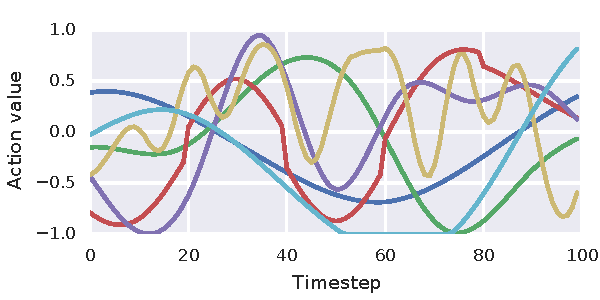
\includegraphics[width=0.4\columnwidth]{figures/random_actions}}
\caption{Sample random sequences obtained from the same distribution than that used to generate random system data to train the models. Sample trajectory video:  \href{\environmentrandomtrajectories}{Video}.}
\label{sm:fig:random_actions}
\end{center}
\vskip -0.2in
\end{figure}

\subsection{Datasets}
\label{sm:sec:data}
For each of the individual fixed systems, we generated 10000 100-step sequences corresponding to about $10^6$ supervised training examples. Additionally, we generated 1000 sequences for validation, and 1000 sequences for testing purposes.

In the case of the parametrized environments, we generated 20000 100-step sequences corresponding to about $2\cdot10^6$ supervised training examples. Additionally, we generated 5000 sequences for validation, and 5000 sequences for testing purposes.

Models trained on multiple environments made use of the corresponding datasets mixed within each batch in equal proportion.


\subsection{Real JACO}
\label{sm:sec:real_jaco}

The real JACO data was obtained under human control during a stacking task. It consisted of 2000 (train:1800, valid:100, test:100) 100-step (timestep 40 ms) trajectories. The instantaneous state of the system was represented in this case by proprioceptive information consisting of joint angles (cosine and sine) and joint velocities for each connected body in the JACO arm, replacing the 13 variables in the dynamic graph.

As the Real JACO observations correspond to the generalized coordinates of the simulated JACO Mujoco model, we use the simulated JACO to render the Real JACO trajectories throughout the paper.

\section{Implementation of the models}
\label{sm:sec:implementation}

\subsection{Framework}
\label{sm:sec:framework}

Algorithms were implemented using TensorFlow and Sonnet. We used custom implementations of the graph networks (GNs) as described in the main text.

\subsection{Graph network architectures}
\label{sm:sec:architectures}
Standard sizes and output sizes for the GNs used are:

\begin{itemize}

\item Edge MLP: 2 or 3 hidden layers. 256 to 512 hidden cells per layer.
\item Node and Global MLP: 2 hidden layers. 128 to 256 hidden cells per layer.
\item Updated edge, node and global size: 128
\item (Recurrent models) Node, global and edge size for state graph: 20
\item (Parameter inference) Node, global and edge size for abstract static graph: 10

\end{itemize}


All internal MLPs used layer-wise ReLU activation functions, except for output layers.

\subsection{Data normalization}
\label{sm:sec:normalization}

The two-layer GN core is wrapped by input and output normalization blocks. The input normalization performs linear transformations to produce a zero-mean, unit-variance distributions for each of the global, node and edge features. It is worth noting that for node/edge features, the same transformation is applied to all nodes/edges in the graph, without having specific normalizer parameters for different bodies/edges in the graph. This allows to reuse the same normalizer parameters regardless of the number and type of nodes/edges in the graph. This input normalization is also applied to the observed dynamic graph in the parameter inference network.  

Similarly, inverse normalization is applied to the output nodes of the forward model, to guarantee that the network only needs to output nodes with zero-mean and unit-variance. 

No normalization is applied to the inferred static graph (from the system identification model), in the output of the parameter inference network, nor the input forward prediction network, as in this case the static graph is already represented in a latent feature space.

\subsection{System invariance}
\label{sm:sec:training_invariance}

When training individual models for systems with translation invariance (Swimmer, Cheetah and Walker2d), we always re-centered the system around 0 before the prediction, and moved it back to its initial location after the prediction. This procedure was not applied when multiple systems were trained together.

\subsection{Prediction of dynamic state change}
\label{sm:sec:delta_prediction}
Instead of using the one-step model to predict the absolute dynamic state, we used it to predict the change in dynamic state, which was then used to update the input dynamic state. For the position, linear velocity, and angular velocity, we updated the input by simply adding their corresponding predicted changes. For orientation, where the output represents the rotation quaternion between the input orientation and the next orientation (forced to have unit norm), we computed the update using the Hamilton product.

\subsection{Forward prediction algorithms}

\subsubsection{One-step prediction}
\label{sm:alg:one_step_prediction}

Our forward model takes the system parameters, the system state and a set of actions, to produce the next system state as explained in SM~Algorithm~\ref{sm:alg:forward_algorithm}.

\begin{algorithm}[tb]
   \caption{Forward prediction algorithm.}
   \label{sm:alg:forward_algorithm}
\begin{algorithmic}
   \STATE {\bfseries Input:}  trained GNs $\textrm{GN}_1$, $\textrm{GN}_2$ and normalizers $\textrm{Norm}_{in}$, $\textrm{Norm}_{out}$.
   \STATE {\bfseries Input:} dynamic state $\textbf{x}^{t_0}$ and actions applied $\textbf{x}^{t_0}$ to a system at the current timestep.
   \STATE {\bfseries Input:} system parameters  $\textbf{p}$
   \STATE Build static graph $G_s$ using $\textbf{p}$
   \STATE Build input dynamic nodes $N^{t_0}_d$ using $\textbf{x}^{t_0}$
   \STATE Build input dynamic edges $E^{t_0}_d$ using $\textbf{a}^{t_0}$
   \STATE Build input dynamic graph $G_d$ using $N^{t_0}_d$ and $E^{t_0}_d$
   \STATE Build input graph $G_i = \textrm{concat}(G_s, G_d)$
   \STATE Obtain normalized input graph $G^n_i = \textrm{Norm}_{in}(G_i)$
   \STATE Obtain graph after the first GN:
   $G^{'}= \textrm{GN}_1(G^n_i)$ 
   \STATE Obtain normalized predicted delta dynamic graph:
   $G^{*}= \textrm{GN}_2(\textrm{concat}(G^n_i, G^{'}))$ 
   \STATE Obtain normalized predicted delta dynamic nodes:
   ${\Delta}N^{n}_d= G^{*}\textrm{.nodes}$  
   \STATE Obtain predicted delta dynamic nodes:
   ${\Delta}N_d = \textrm{Norm}^{-1}_{out}({\Delta}N^{n}_d)$
   \STATE Obtain next dynamic nodes $N^{t_0+1}_d$ by updating $N^{t_0}_d$ with ${\Delta}N_d$
   \STATE Extract next dynamic state $\textbf{x}^{t_0+1}$ from $N^{t_0+1}_d$
   \STATE {\bfseries Output:} next system state $\textbf{x}^{t_0+1}$
\end{algorithmic}
\end{algorithm}


\subsubsection{One-step prediction with System ID}
\label{sm:alg:one_step_prediction_sysid}

\begin{algorithm}[tb]
   \caption{Forward prediction with System ID.}
   \label{sm:alg:sysid_forward}
\begin{algorithmic}
   \STATE {\bfseries Input:} trained parameter inference recurrent GN $\textrm{GN}_p$.
   \STATE {\bfseries Input:} trained GNs and normalizers from Algorithm \ref{sm:alg:forward_algorithm}.
   \STATE {\bfseries Input:} dynamic state $\textbf{x}^{t_0}$ and actions applied $\textbf{x}^{t_0}$ to a parametrized system at the current timestep.
   \STATE {\bfseries Input:} a 20-step sequence of observed dynamic states $x^\textrm{seq}$ and actions $x^\textrm{seq}$ for same instance of the system.
   
   \STATE Build dynamic graph sequence $G^\textrm{seq}_d$ using
   $x^\textrm{seq}_i$ and $a^\textrm{seq}_i$
   \STATE Obtain empty graph hidden state $\textrm{G}_\textrm{h}$.
   \FOR{each graph $G^t_d$ in $G^\textrm{seq}_d$}
   \STATE $\textrm{G}_{o},  \textrm{G}_\textrm{h} = \textrm{GN}_p(\textrm{Norm}_{in}(G^t_d), \textrm{G}_\textrm{h})$,
   \ENDFOR
   \STATE Assign $\textrm{G}_{ID} =\textrm{G}_{o}$
   \STATE Use $\textrm{G}_{ID}$ instead of $G_s$ in Algorithm \ref{sm:alg:forward_algorithm} to obtain $\textbf{x}^{t_0+1}$ from $\textbf{x}^{t_0}$ and $\textbf{x}^{t_0}$
   \STATE {\bfseries Output:} next system state $\textbf{x}^{t_0+1}$
\end{algorithmic}
\end{algorithm}

\begin{algorithm}[t]
   \caption{One step of the training algorithm}
   \label{sm:alg:training_one_step}
\begin{algorithmic}
   \STATE {\bfseries Before training:}  initialize weights of GNs $\textrm{GN}_1$, $\textrm{GN}_2$ and accumulators of normalizers $\textrm{Norm}_{in}$, $\textrm{Norm}_{out}$.
   \STATE {\bfseries Input:} batch of dynamic states of the system $\{\textbf{x}^{t_0}\}$ and actions applied $\{\textbf{a}^{t_0}\}$ at the current timestep
   \STATE {\bfseries Input:} batch of dynamic states of the system at the next timestep $\{\textbf{x}^{t_0+1}\}$ 
   \STATE {\bfseries Input:} batch of system parameters  $\{\textbf{p}_i\}$
   \FOR{each example in batch}
   \STATE Build static graph $G_s$ using $\textbf{p}_i$
   \STATE Build input dynamic nodes $N^{t_0}_d$ using $\textbf{x}^{t_0}$
   \STATE Build input dynamic edges $E^{t_0}_d$ using $\textbf{a}^{t_0}$
   \STATE Build output dynamic nodes $N^{t_0+1}_d$ using $\textbf{x}^{t_0+1}$
   \STATE Add noise to input dynamic nodes $N^{t_0}_d$
   \STATE Build input dynamic graph $G_d$ using $N^{t_0}_d$ and $E^{t_0}_d$
   \STATE Build input graph $G_i = \textrm{concat}(G_s, G_d)$
   
   \STATE Obtain target delta dynamic nodes $\Delta N{'}_{d}$ from $N^{t_0+1}_d$ and $N^{t_0}_d$
   \STATE Update $\textrm{Norm}_{in}$ using $G_i$
   \STATE Update $\textrm{Norm}_{out}$ using ${\Delta}N_{d}$
   
   \STATE Obtain normalized input graph $G^n_i = \textrm{Norm}_{in}(G_i)$
   \STATE Obtain normalized target nodes:
   ${\Delta}N^{n'}_d= \textrm{Norm}_{out}({\Delta}N{'}_{d})$
   \STATE Obtain normalized predicted delta dynamic nodes:
   ${\Delta}N^{n}_d= \textrm{GN}_2(\textrm{concat}(G^n_i, \textrm{GN}_1(G^n_i)))\textrm{.nodes}$  
   \STATE Calculate dynamics prediction loss between ${\Delta}N^{n}_d$ and ${\Delta}N^{n'}_d$.
   \ENDFOR
   \STATE Update weights of $\textrm{GN}_1$, $\textrm{GN}_2$ using Adam optimizer on the total loss with gradient clipping.
\end{algorithmic}
\end{algorithm}

For the System ID foward predictions the model takes a system state and a set of actions for a specific instance of a parametrized system, together with a sequence of observed system states and actions for a for the same system instance. The observed sequence is used to identify the system and then produce the next system state as described in Algorithm \ref{sm:alg:sysid_forward}.


In the case of rollout predictions, the System ID is only performed once, on the provided observed sequence, using the same graph for all of the one-step predictions required to generate the trajectory.

\subsection{Training algorithms}
\label{sm:sec:training}

\subsubsection{One-step}
\label{sm:sec:training_one_step}


We trained the one-step forward model in a supervised manner using algorithm \ref{sm:alg:training_one_step}. Part of the training required finding mean and variance parameters for the input and output normalization, which we did online by accumulating information (count, sum and squared sum) about the distributions of the input edge/node/global features, and the distributions of the change in the dynamic states of the nodes, and using that information to estimate the mean and standard deviation of each of the features.

Due to the fact that our representation of the instantaneous state of the bodies is compatible with configurations where the joint constraints are not satisfied, we need to train our model to always produced outputs within the manifold of configurations allowed by the joints. This was achieved by adding random normal noise (magnitude set as a hyper-parameter) to the nodes of the input dynamic graph during training. As a result, the model not only learns to make dynamic predictions, but to put back together systems that are slightly dislocated, which is key to achieve small rollout errors.


\subsubsection{Abstract parameter inference}
\label{sm:sec:training_inference}

\begin{algorithm}[t]
   \caption{End-to-end training algorithm for System ID.}
   \label{sm:alg:sysid_training}
\begin{algorithmic}
   \STATE {\bfseries Before training:} initialize weights of parameter inference recurrent GN $\textrm{GN}_p$, as well as weights from Algorithm \ref{sm:alg:training_one_step}.
   \STATE {\bfseries Input:} a batch of 100-step sequences with dynamic states $\{x^\textrm{seq}_i\}$ and actions $\{x^\textrm{seq}_i\}$
   \FOR{each sequence in batch}
   \STATE Pick a random 20-step subsequence $x^\textrm{subseq}_i$ and $a^\textrm{subseq}_i$.
   \STATE Build dynamic graph sequence $G^\textrm{subseq}_d$ using
   $x^\textrm{subseq}_i$ and $a^\textrm{subseq}_i$
   \STATE Obtain empty graph hidden state $\textrm{G}_\textrm{h}$.
   \FOR{each graph $G^t_d$ in $G^\textrm{subseq}_d$}
   \STATE $\textrm{G}_{o},  \textrm{G}_\textrm{h} = \textrm{GN}_p(\textrm{Norm}_{in}(G^t_d), \textrm{G}_\textrm{h})$,
   \ENDFOR
   \STATE Assign $\textrm{G}_{ID} =\textrm{G}_{o}$
   \STATE Pick a different random timestep $t_0$ from  $\{x^\mathrm{seq}_i\}$, $\{x^\textrm{seq}_i\}$ 
   \STATE Apply Algorithm \ref{sm:alg:training_one_step} to timestep $t_0$ using final $\textrm{G}_{ID}$ instead $G_s$ to obtain the dynamics prediction loss.
   \ENDFOR
   \STATE Update weights of $\textrm{GN}_p$, $\textrm{GN}_1$, $\textrm{GN}_2$ using Adam optimizer on the total loss with gradient clipping.
\end{algorithmic}
\end{algorithm}

The training of the parameter inference recurrent GN is performed as described in Algorithm \ref{sm:alg:sysid_training}. The recurrent GN and the dynamics GN are trained together end-to-end by sampling a random 20-step sequence for the former, and a random supervised example for the latter from 100-step graph sequences, with a single loss based on the prediction error for the supervised example. This separation between the sequence at the supervised sample, encourages the recurrent GN to truly extract abstract static properties that are independent from the specific 20-step trajectory, but useful for making dynamics predictions under any condition.


\subsubsection{Recurrent one-step predictions}
\label{sm:sec:training_recurrent}

The one-step prediction recurrent model, used for the Real JACO predictions, is trained from 21-step sequences using the \emph{teacher forcing} method. The first 20 graphs in the sequence are used as input graphs, while the last 20 graphs in the sequence are used as target graphs. During training, the recurrent model is used to sequentially process the input graphs, producing at each step a predicted dynamic graph, which is stored, and a graph state, which is fed together with the next input graph in the next iteration. After processing the entire sequence, the sequence of predicted dynamic graphs and the target graphs are used together to calculate the loss.

\subsubsection{Loss}
\label{sm:sec:training_loss}
We use a standard L2-norm between the normalized expected and predicted delta nodes, for the position, linear velocity, and angular velocity features. We do this for the normalized features to guarantee a balanced relative weighting between the different features. In the case of the orientation, we cannot directly calculate the L2-norm between the predicted rotation quaternion $\textbf{q}_p$ to the expected rotation quaternion $\textbf{q}_e$, as a quaternion $\textbf{q}$ and $-\textbf{q}$ represent the same orientation. Instead, we minimize the angle distance between $\textbf{q}_p$ and $\textbf{q}_e$ by minimizing the loss $1-\cos^2{(\textbf{q}_e\cdotp\textbf{q}_p)}$ after.

\subsection{Training details}
\label{sm:sec:training_details}

Models were trained with a batch size of 200 graphs/graph sequences, using an Adam optimizer on a single GPU. Starting learning rates were tuned at $1^{-4}$. We used two different exponential decay with factor of 0.975 updated every 50000 (fast training) or 200000  (slow training) steps.

We trained our models using early stopping or asymptotic convergence based the rollout error on 20-step sequences from the validation set. Simple environments (such as individual fixed environments) would typically train using the fast training configuration for a period between less than a day to a few days, depending on the size of the environment and the size of the network. Using slow training in these cases only yields a marginal improvement. On the other hand, more complex models such as those learning multiple environments and multiple parametrized environments benefited from the slow training to achieve optimal behavior for periods of between 1-3 weeks.

\section{MLP baseline architectures}
\label{sm:sec:MLP baseline}

For the MLP baselines, we used 5 different models (ReLU activation) spanning a large capacity range:
\begin{itemize}
    \item 3 hidden layers, 128 hidden cells per layer
    \item 3 hidden layers, 512 hidden cells per layer
    \item 9 hidden layers, 128 hidden cells per layer
    \item 9 hidden layers, 512 hidden cells per layer
    \item 5 hidden layers, 256 hidden cells per layer
\end{itemize}

The corresponding MLP replaces the 2-layer GN core, with additional layers to flatten the input graphs into feature batches, and to reconstruct the graphs at the output. Both normalization and graph update layers are still applied at graph level, in the same way that for the GN-based model.

Each of the models was trained four times using initial learning rates of $1^{-3}$ and $1^{-4}$ and learning rate decays every 50000 and 200000 steps. The model performing best on validation rollouts for each environment, out of the 20 hyperparameter combinations was chosen as the MLP baseline.

\section{Control}
\label{sm:sec:control}

\subsection{Model-based planning algorithms}
\label{sm:sec:model_based_planning}

\subsubsection{MPC planner with learned models}
\label{sm:sec:planning_mpc}

\begin{algorithm}[tb]
   \caption{MPC algorithm}
   \label{sm:alg:MPC}
\begin{algorithmic}
   \STATE {\bfseries Input:} initial system state $\textbf{x}^{0}$,
   \STATE {\bfseries Input:} randomly initialized sequence of actions $\{\textbf{a}^{t}\}$.
   \STATE {\bfseries Input:} pretrained dynamics model $M$ such
   
   $\textbf{x}^{t_0+1} = M(\textbf{x}^{t_0}, \textbf{a}^{t_0})$
   \STATE {\bfseries Input:}  Trajectory cost function $L$ such
   
   $c = C(\{\textbf{x}^{t}\}, \{\textbf{a}^{t}\})$
   \FOR{a number of iterations}
   \STATE $\textbf{x}^{0}_r=\textbf{x}^{0}$
   \FOR{t in range(0, horizon)}
     \STATE $\textbf{x}^{t+1}_r=M(\textbf{x}^{t}_r, \textbf{a}^{t})$
   \ENDFOR
   \STATE Calculate trajectory cost $c = C(\{\textbf{x}_r^{t}\}, \{\textbf{a}^{t}\})$
   \STATE Calculate gradients $\{\textbf{g}_a^{t}\} = \frac{\partial c}{\partial \{\textbf{a}^{t}\}}$
   \STATE Apply gradient based update to $\{\textbf{a}^{t}\}$
   \ENDFOR
   \STATE {\bfseries Output:} optimized action sequence $\{\textbf{a}^{t}\}$ 
\end{algorithmic}
\end{algorithm}

We implemented MPC using our learned models as explained in SM~Algorithm~\ref{sm:alg:MPC}. We applied the algorithm in a receding horizon manner by iteratively planning for a fixed horizon (see SM~Table~\ref{sm:sec:planning_configuration}), applying the first action of the sequence, and increasing the horizon by one step, reusing the shifted optimal trajectory computed in the previous iteration. We typically performed between 3 and 51 optimization iterations $N$ from each initial state, with additional $N\cdot \textrm{horizon}$ iterations at the very first initial state, to \emph{warm-up} the fully-random initial action sequence.


\subsubsection{Baseline Mujoco-based planner}
\label{sm:sec:planning_mujoco_baseline}

As a baseline planning approach we used the iterative Linear-Quadratic-Gaussian (iLQG) trajectory optimization approach proposed in \cite{tassa2014control}.  This method alternates between forward passes (rollouts) which integrate the dynamics forward for a current control sequence and backwards passes which consists of perturbations to the control sequence to improve upon the recursively computed objective function.  
Note that in the backwards pass, each local perturbation can be formulated as an optimization problem, and linear inequality constraints ensure that the resulting control trajectory does not require controls outside of the range that can be feasibly generated by the corresponding degrees of freedom in the MuJoCo model.
The overall objective optimized corresponds to the total cost over $J$ a finite horizon:
\begin{equation}
    J(x_0, U) = \sum_{t=0}^{T-1} \ell (x_t, u_t) + \ell (x_T)
\end{equation}
where $x_0$ is the initial state, $u_t$ is the control signal (i.e. action) taken at timestep $t$, $U$ is the trajectory of controls, $\ell(\cdot)$ is the cost function.  We assume the dynamics are deterministic transitions $x_{t+1} = f(x_t, u_t)$. 

While this iLQG planner does not work optimally when the dynamics involve complex contacts, for relatively smooth dynamics as found in the swimmer, differential dynamic programming (DDP) style approaches works well \cite{tassa2008receding}.  Relevant cost functions are presented in SM~Section~\ref{sm:sec:planning_configuration}. 

\subsection{Planning configuration}
\label{sm:sec:planning_configuration}

\vskip 0.15in
\begin{center}
\begin{small}
\renewcommand{\arraystretch}{1.5}
\begin{tabular}{p{15mm}p{30mm}p{15mm}p{90mm}}
\toprule
 Name & Task & Planning \newline horizon & Reward to maximize (summed for all timesteps) \\
\midrule
Pendulum  & Balance & 50, 100 & Negative angle between the quaternion of the pendulum and the target quaternion corresponding to the balanced position. (0 when balanced at the top, $<0$ otherwise).
\\
Cartpole  & Balance & 50, 100 & Same as Pendulum-Balance calculated for the pole.\\
Acrobot   & Swing up & 100 & Same as Pendulum-Balance summed for both acrobot links.\\
Swimmer   & Mover towards target & 100 & Projection of the displacement vector of the Swimmer head from the previous timestep on the target direction, The target direction is calculated as the vector joining the head of the swimmer at the first planning timestep with the target location. The reward is shaped (0.01 contribution) with the negative squared projection on the perpendicular target direction.\\
Cheetah   & Move forward & 20 & Horizontal component of the absolute velocity of the torso.\\
   & Vertical position & 20 & Vertical component of the absolute position of the torso.\\
   & Squared vertical speed &20 & Squared vertical component of the absolute velocity of the torso.\\
   & Squared angular speed & 20& Squared angular velocity of the torso.\\
Walker2d   & Move forward &20 & Horizontal component of the absolute velocity of the torso.\\
   & Vertical position &20 & Vertical component of the absolute position of the torso.\\
   & Inverse verticality &20& Same as Pendulum-Balance summed for torso, thighs and legs.\\
   & Feet to head height &20& Summed squared vertical distance between the position of each of the feet and the height of Walker2d.\\
Jaco      & Imitate Palm Pose &20& Negative dynamic-state loss (as described in Section \ref{sm:sec:training_loss}) between the position-and-orientation of the body representing the JACO palm and the target position-and-orientation .\\
  & Imitate Full Pose &20& Same as Jaco-Imitate Palm Pose but summed across all the bodies forming JACO (see SM~Section~\ref{sm:sec:training_loss}).\\


\bottomrule
\end{tabular}
%\end{sc}
\end{small}
\end{center}
\vskip -0.1in
\renewcommand{\arraystretch}{1.}



\subsection{Reinforcement learning agents}
\label{sm:sec:reinforcement_learning}
Our RL experiments use three base algorithms for continuous control: DDPG \citep{Lillicrap16}, SVG(0) and SVG(N)~\citep{heess2015learning}. All of these algorithms find a policy $\pi$ that selects an action $a$ in a given state $x$ by maximizing the expected discounted reward,
\begin{equation}
Q(\mathbf{x}, \mathbf{a}) = \mathbb{E} \Big[ \sum_{t=0}^\infty \gamma^t r(\mathbf{x}, \mathbf{a}) \Big],
\end{equation}
where $r(x,a)$ is the per-step reward and $\gamma$ denotes the discount factor.
Learning in all algorithms we consider occurs off-policy. That is, we continuously generate experience via the current best policy $\pi$, storing all experience (sequences of states, actions and rewards) it into a replay buffer $\mathcal{B}$, and minimize a loss defined on samples from $\mathcal{B}$ via stochastic gradient descent.


\subsubsection{DDPG}
\label{sm:sec:ddpg}
The DDPG algorithm~\citep{Lillicrap16} learns a deterministic control policy $\pi = \mu_\theta(s)$ with parameters $\theta$ and a corresponding action-value function $Q_\phi^\mu(s, a)$, with parameters $\phi$. Both of these mapping are parameterized via neural networks in our experiments.

Learning proceeds via gradient descent on two objectives. The objective for learning the $Q$ function is to minimize the one-step Bellman error using samples from a replay buffer, that is we seek to find $\arg \min_\phi L(\phi)$ by following the gradient,
\begin{equation}
\begin{aligned}
\nabla_\phi L(\phi) &= \mathbb{E}_{(\mathbf{x}_t, \mathbf{a}_t, \mathbf{x}_{t+1}, r_t) \in \mathcal{B}} \Big[ \nabla_\phi \big( Q^\mu_\phi(\mathbf{x}_t, \mathbf{a}_t) - y \big)^2\Big], \\
\text{with } \ y &= r_t + \gamma Q^\mu_{\phi'}(\mathbf{x}_{t+1}, \mu_{\theta'}(\mathbf{x}_{t+1}))
\end{aligned}
\label{eq:q_learning}
\end{equation}
where $\phi'$ and $\theta'$ denote the parameters of target Q-value and policy networks, that are periodically copied from the current parameters, this is common practice in RL to stabilize training (we update the target networks every $1000$ gradient steps).
The objective for learning the policy is performed by searching for an action that obtains maximum value, as judged by the learned Q-function. That is we find $\arg \min_\theta L(\theta)$ by following the deterministic policy gradient \cite{Lillicrap16},
\begin{equation}
\nabla_\theta L^{\text{DPG}}(\theta) = \mathbb{E}_{\mathbf{x}_t \in \mathcal{B}} \Big[ - \nabla_\theta Q^\mu_\theta(\mathbf{x}_t, \mu_\theta(\mathbf{x}_t))\Big].
\label{eq:ddpg_grad}
\end{equation}

\subsubsection{SVG}
\label{sm:sec:svg}
For our experiments with the familiy of Stochastic Value Gradient (SVG) \citep{heess2015learning} algorithms we considered two-variants a model-free baseline SVG(0) that optimizes a stochastic policy based on a learned Q-function as well as a model-based version SVG(N) (using our Graph Net model) that unrolls the system dynamics for N-steps.

\paragraph{SVG(0)} In the model-free variant learning proceeds similarly to the DDPG algorithm. We learn both, a parametric Q-value estimator as well as a (now stochastic) policy $\pi_\theta(\mathbf{a} | \mathbf{x})$ from which actions can be sampled. 
In our implementation learning of the Q-function is performed by following the gradient from Equation \eqref{eq:q_learning}, with $\mu(x)$ replaced by samples $\mathbf{a} \sim \pi_\theta(\mathbf{a} | \mathbf{x})$. 

For the policy learning step we can learn via a stochastic analogue of the deterministic policy gradient from Equation \eqref{eq:ddpg_grad}, the so called stochastic value gradient, which reads
\begin{equation}
\nabla_\theta L^{\text{SVG}}(\theta) = - \nabla_\theta \mathbb{E}_{\substack{\mathbf{x}_t \in \mathcal{B} \\ \mathbf{a} \sim \pi_\theta(\mathbf{a} | \mathbf{x}_t)}} \Big[ Q^\pi_\theta(\mathbf{x}_t, \cdot)\Big].
\label{eq:svg0}
\end{equation}
For a Gaussian policy (as used in this paper) the gradient of this expectation can be calculated via the reparameterization trick \citep{Kingma2013auto,rezende14}.


\paragraph{SVG(N)}
For the model based version we used a variation of SVG(N) that employs an action-value function -- instead of the value function estimator used in the original paper. This allowed us to directly compare the performance of a SVG(0) agent, which is model free, with SVG(1) which calculates policy gradients using a one-step model based horizon. 

In particular, similar to Equation \eqref{eq:svg0}, we obtain the model based policy gradient as 
\begin{equation}
\nabla_\theta L^{\text{SVG(N)}}(\theta) = - \nabla_\theta \mathbb{E}_{
\substack{\mathbf{x}_t \in \mathcal{B} \\ 
 %\mathbf{x}_{t+1} \sim p(\mathbf{x} | \mathbf{x}_t, \mathbf{a}_t) \\ 
 \mathbf{a}_t \sim \pi_\theta(\mathbf{a} | \mathbf{x}_t)\\ 
 \mathbf{a}_{t+1} \sim \pi_\theta(\mathbf{a} | \mathbf{x}_{t+1})}} \Big[ r_{t}(\mathbf{x}_t, \mathbf{a}_t) + \gamma Q^\pi_\theta(\mathbf{x}_{t+1}, \mathbf{a}_t) \mid \mathbf{x}_{t+1} = g(\mathbf{x}_t, \mathbf{a}_t) \Big],
\end{equation}
where $g$ denotes the dynamics, as predicted by the GN and the gradient can, again, be computed via reparameterization (we refer to \citet{heess2015learning} for a detailed discussion).

We experimented with SVG(1) on the swimmer domain with six links (Swimmer 6). Since in this case, the goal for the GN is to predict environment observations (as opposed to the full state for each body), we constructed a graph from the observations and actions obtained from the environment.
SM Figure \ref{sm:fig:swimmer_graph_conversion} describes the observations and actions and shows how they were transformed into a graph.


\section{Mujoco variables included in the graph conversion}
\label{sm:sec:mujoco_variables}

\subsection{Dynamic graph}

We retrieved the the absolute position, orientation, linear and angular velocities for each body:
\begin{itemize}
\item \textbf{Global: None}
\item \textbf{Nodes:} (for each body)\\
Absolute body position (3 vars): mjData.xpos \\
Absolute body quaternion orientation position (4 vars): mjData.xquat \\
Absolute linear and angular velocity (6 vars): mj\_objectVelocity
(mjOBJ\_XBODY, flg\_local=False)
\item \textbf{Edges:} (for each joint) Magnitude of action at joint: mjData.ctrl (0, if not applicable).
\end{itemize}

\subsection{Static graph}
We performed an exhaustive selection of global, body, and joint static properties from mjModel:
\begin{itemize}
\item \textbf{Global:} mjModel.opt.\{timestep, gravity, wind, magnetic, density, viscosity, impratio, o\_margin, o\_solref, o\_solimp, collision\_type (one-hot), enableflags (bit array), disableflags (bit array)\}.
\item \textbf{Nodes:} (for each body) mjModel.body\_\{mass, pos, quat, inertia, ipos, iquat\}.
\item \textbf{Edges:} (for each joint) \\Direction of edge (1: parent-to-child, -1: child-to-parent). \\Motorized flag (1: if motorized, 0 otherwise). \\Joint properties: mjModel.jnt\_\{type (one-hot), axis, pos, solimp, solref, stiffness, limited, range, margin\}. \\Actuator properties: mjModel.opt.actuator\_\{biastype (one-hot), biasprm, cranklength, ctrllimited, ctrlrange, dyntype (one-hot), dynprm, forcelimited, forcerange, gaintype (one-hot), gainprm, gear, invweight0, length0, lengthrange\}.
\end{itemize}

Most of these properties are constant for all environments use, however, they are kept for completeness. While we do not include geom properties such as size, density or shape, this information should be partially encoded in the inertia tensor together with the mass.

\section{Supplementary figures}
\label{sm:sec:supplementary_figures}

\begin{figure}[ht]
\vskip 0.2in
\begin{center}
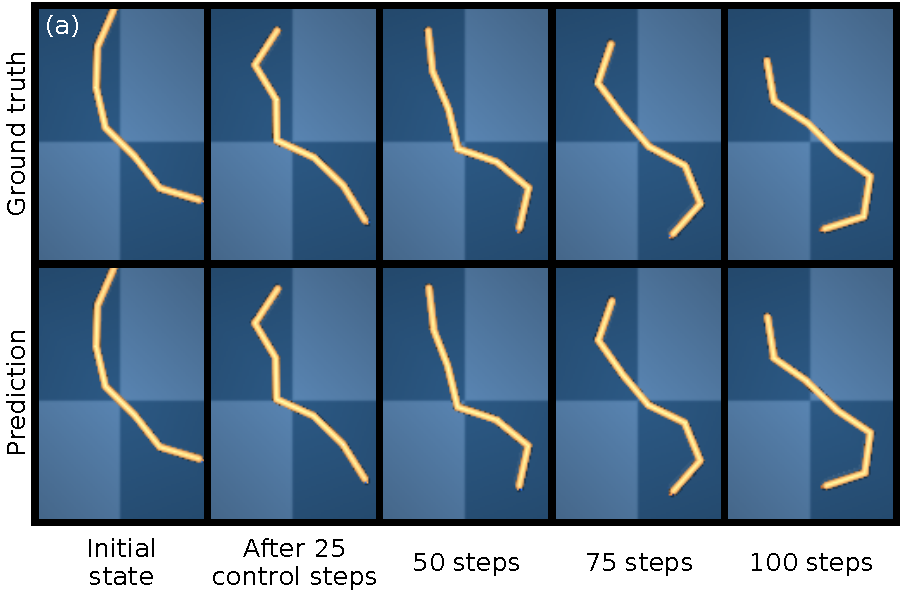
\includegraphics[width=0.45\columnwidth]{figures/swimmer_rollout_frames_dpg}
\hspace{0.2cm}
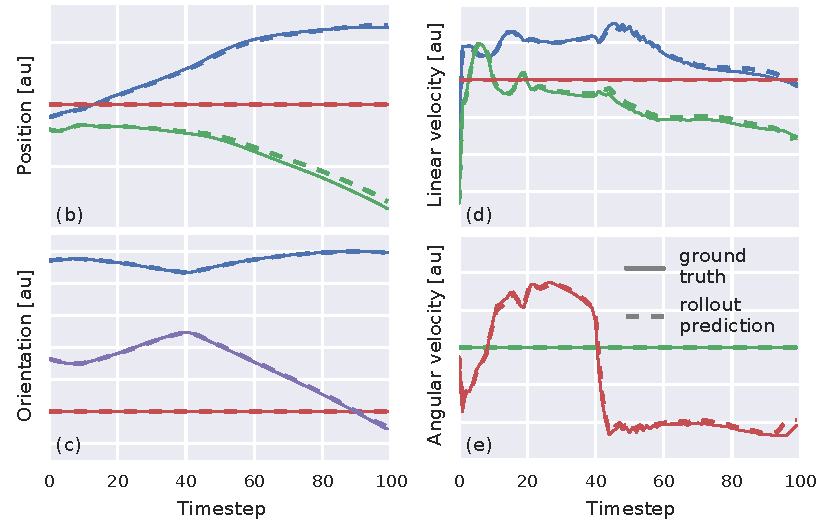
\includegraphics[width=0.46\columnwidth]{figures/swimmer_rollout_dpg}
\caption{Model trained on Swimmer6 trajectories under random control evaluated on a trajectory generated by a DDPG agent. Trajectories are also available in video [\href{\rolloutsswimmerdpgdata}{\rolloutsswimmerdpgdataname}]. 
(Left) Key-frames comparing the ground truth and predicted sequence within a 100 step trajectory. (Right) Full state sequence prediction for the third link of the Swimmer, consisting of Cartesian position (3 vars), quaternion orientation (4 vars), Cartesian linear velocity (3 vars) and Cartesian angular velocity (3 vars). The full prediction contains such 13 variables for each of the links, that is 78 variables.
}
\label{sm:fig:swimmer_rollout_dpg}
\end{center}
\vskip -0.2in
\end{figure}

\begin{figure}[ht]
\vskip 0.2in
\begin{center}
\centerline{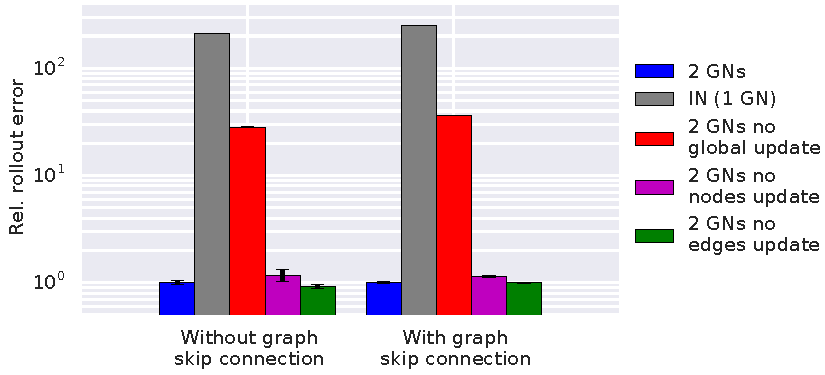
\includegraphics[width=0.5\columnwidth]{figures/ablation_study}}
\caption{Ablation study of the architecture using the rollout error over 20 step test sequences in Swimmer6 to evaluate relative performance. The performance of the architecture used in this work (a sequence of two GNs, blue) is compared to: an Interaction Network (IN) \cite{battaglia2016interaction}, which is equivalent in this case to a single GN (grey), and a sequence of GNs where the first GN is not allowed to update either the global (red), the nodes (purple) or the edges(green) of the output graph. Results are shown both for a purely sequential connection of the GNs, and for a model with a graph skip connection, where the output graph of the first GN, is concatenated to the input graph, before feeding it into the second GN. The results show that the performance of the double GN is far superior than that of the equivalent IN. They also show that the global update performed by the GN is necessary for the model to perform well. We hypothesize this is due to the long range dependencies within the graph that exist within swimmer, and the ability of the global update to quickly propagate such dependencies across the entire graph. Similar results may have been obtained without global updates by using a deeper stack of GNs to allow information to flow across the entire graph.
Each model was trained from three different seeds. The figure depicts the mean, and the standard deviation of the asymptotic performance of the three seeds.}
\label{sm:fig:ablation_study}
\end{center}
\vskip -0.2in
\end{figure}

\begin{figure}[ht]
\vskip 0.2in
\begin{center}
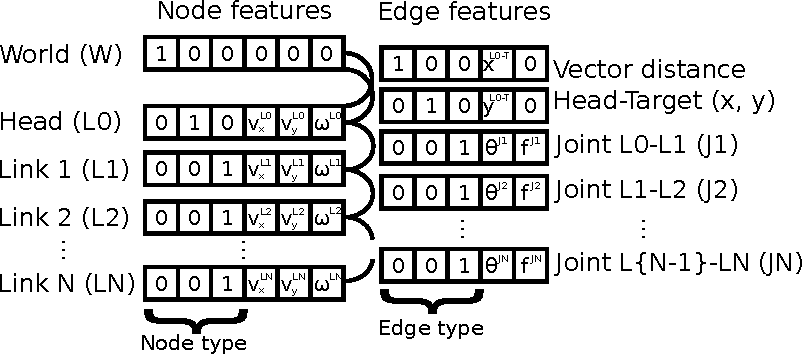
\includegraphics[width=0.6\columnwidth]{figures/swimmer_graph_conversion}
\caption{Arrangement as a graph of the default 25-feature observation and 5 actions provided in the Swimmer 6 task from the DeepMind Control Suite \cite{tassa2018deepmind}. The observation consists of: \emph{(to\_target)} the distance between the head and the target projected in the axis of the head ($x^{\text{L0-T}}$, $y^{\text{L0-T}}$), \emph{(joints)} the angle of each joint JN between adjacent swimmer links L{N-1} and L{N} ($\theta^{\text{JN}}$) and \emph{(body\_velocities)} the linear and angular velocity of each link LN projected in its own axis ($v_x^{\text{LN}}$, $v_y^{\text{LN}}$, $\omega^{\text{LN}}$). The actions consists of the force applied to each of the joints ($f^\text{JN}$) connecting the links. Because our graphs are directed, all of the edges were duplicated, with an additional {-1, 1} feature indicating the direction.}
\label{sm:fig:swimmer_graph_conversion}
\end{center}
\vskip -0.2in
\end{figure}